\section{Experiments}
\label{sec:experiments}
\suppressfloats[t]
We provide empirical support for each claim in \S\ref{sec:grpo}--\S\ref{sec:method} through a corresponding table or figure. Unless otherwise noted, diagnostics use Game24, which shows the largest gap between variants; results for other tasks appear in Appendix~\ref{app:results}.

\paragraph{Setup.}
We evaluate on four program-verified tasks: \textbf{Countdown}, \textbf{Sudoku}, \textbf{Knights-and-Knaves} (K\&K) and \textbf{Game24} (Appendix~\ref{app:datasets}). All runs start from ELF-B (105M) fine-tuned separately on each task, serving as the base. We write $\gamma a$\texttt{@}$K$ for a $K$-step stochastic chain with churn $\gamma=a$. Accuracy is measured on 2{,}000 held-out prompts (1{,}601 for Game24) using both the deployment chain ($\gamma56$@64; $\gamma28$@32 on Sudoku) and a cheaper chain ($\gamma4$@16; $\gamma14$@16 on Sudoku). \methodGRPO{} is trained under the cheap chain with 128 rollouts per iteration for 600 iterations. Both SVG variants follow Algorithm~\ref{alg:jpc} under the deployment chain for 1{,}000--1{,}500 iterations. As cross-architecture references, we train GPT-2 (124M) with GRPO/PPO and LLaDA-8B-Instruct with diffu-GRPO \citep{zhao2025d1} on the same data. We report each each model's best held-out checkpoints over its own evaluation grid. Appendix~\ref{app:details} provides more details.

\begin{table}[t]
\centering\small
\begin{minipage}[c]{0.60\linewidth}
\centering
\setlength{\tabcolsep}{3pt}
\resizebox{\linewidth}{!}{%
\begin{tabular}{@{}lcccc@{}}
\toprule
 & Countdown & Sudoku & K\&K & Game24 \\
\midrule
\multicolumn{5}{@{}l}{\emph{GPT-2 (124M, autoregressive)}}\\
task SFT & 44.2 & \phantom{0}1.2 & 92.9 & 26.9 \\
+ token GRPO/PPO & 53.9 (+9.7) & \phantom{0}1.4 (+0.2) & 93.2 (+0.3) & 32.2 (+5.3) \\
\midrule
\multicolumn{5}{@{}l}{\emph{LLaDA-8B-Instruct (8B, masked diffusion)}}\\
task SFT & 13.1 & \phantom{0}0.7 & 61.0 & 16.1 \\
+ diffu-GRPO & 14.9 (+1.8) & \phantom{0}0.7 (+0.0) & 62.5 (+1.5) & 19.5 (+3.4) \\
\midrule
\multicolumn{5}{@{}l}{\emph{ELF-B (105M, continuous flow)}}\\
task SFT (base) & 42.2 & 66.2 & 67.5 & 45.0 \\
+ \methodGRPO & 43.1 (+0.9) & 69.7 (+3.5) & 71.6 (+4.1) & 47.5 (+2.5) \\
+ \methodSVGScalar{} & 48.2 (+6.0) & 66.3 (+0.1) & 77.6 (+10.1) & 51.4 (+6.4) \\
+ \hl{\methodSVGTwoD{}} & \textbf{50.2 (+8.0)} & \textbf{71.0 (+4.8)} & \textbf{79.6 (+12.1)} & \textbf{58.8 (+13.8)} \\
\bottomrule
\end{tabular}}
\end{minipage}\hfill
\begin{minipage}[c]{0.385\linewidth}
\centering
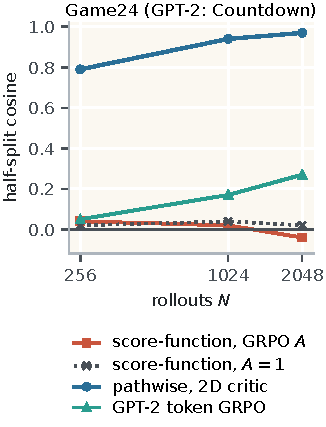
\includegraphics[width=\linewidth]{figures/fig_estimator.pdf}
\end{minipage}
\caption{\textbf{Left:} held-out accuracy (\%) under the deployment chain; ELF\mbox{-}B RL rows are means of three seeds (Appendix~\ref{app:seeds}), other rows single runs; bold: best ELF\mbox{-}B row per column. \textbf{Right, top:} half-split cosine of the gradient on rollouts of the base at flow step 24 of 64 (GPT-2: Countdown, its own sampler). \textbf{Right, bottom:} change in held-out accuracy after \emph{one} step from the base along the mean gradient of $1{,}024$ rollouts,  against the step's length.}
\label{tab:main}
\end{table}

% : score-function with the GRPO advantage (\lk{cgrpo}) and with the $A{=}1$ control (\lk[densely dotted]{cctrl}), pathwise through the pre-trained 2D critic (\lk{ctwod}), GPT-2's token-level GRPO (\lk{cgpt}); mean of 10 random splits (sd $\le0.05$)
% in AdamW's per-coordinate normalised form,
% in units of $D$, the distance $750$ training iterations travel
% : pathwise (\lk{ctwod}), score-function (\lk{cgrpo}), random direction (\lk[densely dotted]{cctrl})

\subsection{Main result}
\label{sec:exp_main}
Table~\ref{tab:main} shows consistent improvement across the ELF-B variants for three out of four datasets. GRPO provides modest gains, while the scalar-critic pathwise update improves Countdown, K\&K, and Game24 by 6--10 points. The 2D critic performs best on every task and varies by about one point across seeds. The scalar critic is less stable: on Sudoku, the held-out accuracy remains near the base and declines after its first checkpoint. The GPT-2 results show that score-function RL improves a similarly sized AR model by nearly ten points on Countdown, compared with one point for the flow model. Diffu-GRPO improves LLaDA by at most three points despite its larger scale and lower baseline accuracy. These results serve as cross-architecture references for the estimator rather than direct comparisons of model capability (Appendix~\ref{app:d1}).

\subsection{From GRPO to SVG: Why the score-function variant is capped}
\label{sec:exp_estimator}
Refining the advantage does not improve the flow model's GRPO by more than five points (Appendix~\ref{app:sf_variants}), nor does training with the deployment chain instead of the cheap chain (Appendix~\ref{app:grpo_chain}). Although GRPO requires three to five times fewer denoiser calls than Algorithm~\ref{alg:jpc}, even a 16-fold larger batch provides little additional signal (Table~\ref{tab:main} top right panel). Its limiting factor is the action space: one reward must supervise $(K-2)\,|\mathcal G|\,d$ Gaussian coordinates.

The top right panel of Table~\ref{tab:main} compares estimator variance by splitting $N$ Game24 rollouts into two halves and measuring the cosine similarity between their mean gradients; greater agreement indicates a more reproducible signal. The $A{=}1$ control provides a zero-mean noise floor. The flow model's score-function gradient remains near this floor even at $N{=}2048$, equivalent to sixteen GRPO batches. GPT-2's token-level gradient separates from the floor as $N$ increases, showing that the same estimator is more effective for semantic token decisions. In contrast, the pathwise gradients agree strongly from $N{=}256$. The bottom-right panel tests whether these directions improve the policy by taking one AdamW-normalized step from the base along each estimated gradient and reevaluates the same held-out prompts with matched sampling noise. The pathwise step substantially improves accuracy, whereas the score-function step computed from the same rollouts is indistinguishable from a random direction. The pathwise direction is therefore both reproducible and effective under optimizer normalization. Without normalization, its magnitude is concentrated in roughly one percent of the parameters and degrades the policy despite increasing critic value (Appendix~\ref{app:onestep}). Performance declines at the largest step size because the update moves beyond the region where the frozen critic is reliable, motivating the jointly updated critic studied in \S\ref{sec:exp_critic}.

\begin{table}[!t]
\centering\small
\begin{minipage}[c]{0.565\linewidth}
\centering
\setlength{\tabcolsep}{3pt}
\resizebox{\linewidth}{!}{%
\begin{tabular}{@{}lcccc@{}}
\toprule
critic & Pearson $r$ & pick@$V$ & best & final \\
\midrule
fine-tuned copy, reads $(y_k,\hat x_{k-1})$ & \CDa{1} & \CDa{3} & \CDa{5} & \CDa{6} \\
\quad without $\hat x_{k-1}$ in the input & \CDb{1} & \CDb{3} & \CDb{5} & \CDb{6} \\
\quad copy frozen in pre-training & \CDc{1} & \CDc{3} & \CDc{5} & \CDc{6} \\
\quad random initialisation & \CDd{1} & \CDd{3} & 37.9 & \phantom{0}4.1 \\
\quad copy also trained in RL & \CDa{1} & \CDa{3} & 49.7 & 49.3 \\
\quad frozen in RL$^\dagger$ & --- & --- & 48.4 & \phantom{0}0.3 \\
\bottomrule
\end{tabular}}
\end{minipage}\hfill
\begin{minipage}[c]{0.42\linewidth}
\centering
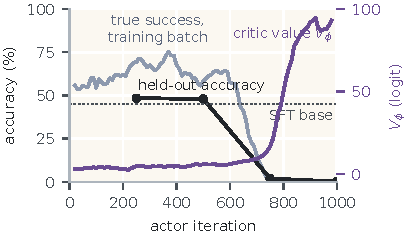
\includegraphics[width=\linewidth]{figures/fig_frozen.pdf}
\end{minipage}
\caption{\textbf{Left:} critic design on Game24, one element changed per row; bold: the critic of Algorithm~\ref{alg:jpc}. \emph{Offline} (held-out rollouts of the base, deployment chain, step 32 of 64): correlation of the pooled value with the outcome, and pick@$V$, the success rate of the top-ranked of eight rollouts (chance $0.55$). \emph{Online}: held-out accuracy (\%) of one run with that critic, best and final checkpoint. \textbf{Right:} the last row over training ($^\dagger$earlier recipe, Appendix~\ref{app:details}).}
\label{tab:critic_design}
\end{table}

% (---: not run)
% : success of the training batch (\lkn{cgrey}, smoothed), held-out accuracy (\lk{cblack}), the critic's pooled value on that batch (\lkn{cpurple}, logits, right axis); dotted: the base

\subsection{Training the critics jointly with the actor}
\label{sec:exp_critic}
Table~\ref{tab:critic_design} evaluates critic variants both offline and online; the two evaluations give the same ranking. The full critic in Algorithm~\ref{alg:jpc} (first row) predicts outcomes well and reaches the performance reported in Table~\ref{tab:main}. Removing self-conditioning $\hat x_{k-1}$ from its input or freezing the denoiser copy during pre-training reduces offline correlation by one-third to one-half. The online policies improve briefly and then collapse. A randomly initialized copy performs worse and never exceeds the base. During RL, however, only the critic head should be updated. Updating the full critic under the limited online budget degrades its pretrained features and reduces policy improvement (Appendix~\ref{app:critic_training}). The last row of Table~\ref{tab:critic_design}, traced over training in the right panel, shows why the critic must continue adapting. Freezing the entire critic initially improves the policy, but the critic eventually becomes stale and exploitable. Between iterations 500 and 750, its predicted value approaches certainty while training and held-out accuracy collapse. Refitting the head (\S\ref{sec:joint}) repairs this failure but cannot compensate for features that do not encode the outcome.

\begin{figure}[t]
\centering
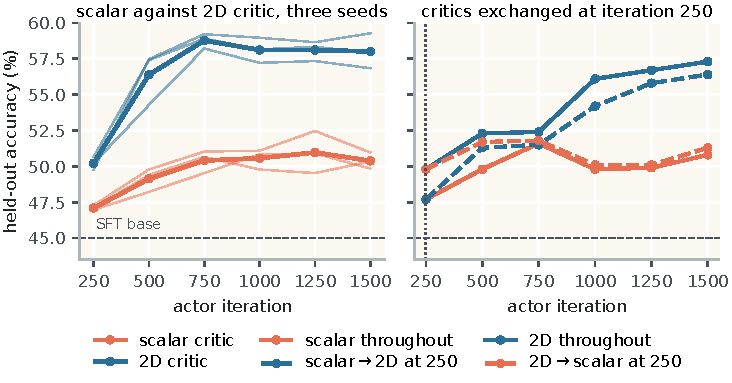
\includegraphics[width=\linewidth]{figures/fig_dyn.pdf}
\caption{Game24, held-out accuracy (\%) under the deployment chain. \textbf{Left:} the runs of Table~\ref{tab:main} after that many actor iterations, three seeds (thin) and their mean (thick). \textbf{Right:} a fourth seed of each recipe stopped at iteration 250 (dotted vertical) and continued with its own critic (solid) or with the other recipe's pre-trained critic, refit from 250 on.}
\label{fig:dyn}
\end{figure}

% ; scalar critic~\lk{cscalar}, 2D critic~\lk{ctwod}
% (dashed: \lk[dashed]{ctwod}~scalar-trained policy under the 2D critic, \lk[dashed]{cscalar}~2D-trained policy under the scalar critic); colour marks the critic in charge after the exchange. Both panels: dashed grey, the base. Values in Appendix~\ref{app:swap_late}

\subsection{The 2D critic keeps the update improving}
\label{sec:exp_2d}
The left panel of Figure~\ref{fig:dyn} shows similar early progress for the scalar and 2D critics. After roughly 500 iterations, the scalar policy plateaus or declines, whereas the 2D policy improves through iteration 750 and retains its gains. This pattern holds on Game24, Countdown, and K\&K (Appendix~\ref{app:traj}). Sudoku is the exception: both variants decline early, and the reported $71.0$ in Table~\ref{tab:main} is the 500-iteration checkpoint.

The 2D critic's advantage does not appear in static evaluation, but in joint training. On states from the same policy, the two critics predict outcomes equally well, respond similarly to an isolated token error, and refit equally stably (Appendix~\ref{app:critic_equiv}). In the right panel, we exchange the critics at iteration 250, while the policies are still close. Thereafter, performance follows the critic: the scalar-trained policy approaches the full 2D run after switching to the 2D critic, whereas the 2D-trained policy plateaus after switching to the scalar critic. A swap at iteration 750 has little effect because the learning rate and policy movement are already small (Appendix~\ref{app:swap_late}). Thus, the 2D critic's benefit lies in guiding the policy as it evolves. Two observations further localize the this advantage to critic refitting: a frozen 2D critic is exploited as quickly as a frozen scalar critic, while scalar-head discrimination declines on Countdown but not Sudoku (Appendix~\ref{app:critic_equiv}; Appendix~\ref{app:traj}).

Two components jointly explain the 2D critic's advantage: position-specific gradients from the head-before-mean architecture and per-position supervision during critic refitting. On Game24, architecture alone suffices: exchange runs improve while refitting the 2D critic using only the pooled loss, as each position receives the head's slope at its own feature rather than at the mean~(\ref{eq:headgrad}). On Countdown, this alone is insufficient: removing per-position supervision reduces performance to the scalar-critic's level, while quadrupling refitting steps for scalar-critic does not help. The per-position term in~(\ref{eq:critic2d_loss}) keeps the value field informative as the policy evolves (Appendix~\ref{app:needs_full}).

\subsection{Ablations}
\label{sec:ablations}
Table~\ref{tab:needs} isolates the main design choices in Algorithm~\ref{alg:jpc}. For the actor objective, log-odds outperform probability (\S\ref{sec:pathwise}) , while mean pooling outperforms minimum pooling (\S\ref{sec:jpc_2d}). Refitting the head at the top of the actor window is especially important on Countdown, where earlier states reveal little about the final outcome (\S\ref{sec:joint}). A decaying actor learning rate keeps the final accuracy of every 2D-critic seed within 1.5 points of its peak on Countdown, K\&K and Game24; a constant rate declines, and a three-times-larger rate collapses, consistent with the accumulated bias. Finally, improvements remain tied to the training chain: a policy trained with the cheap chain performs nine points worse under the deployment chain than the same method trained there, motivating the amortisation loop.
\begin{table}[!ht]
\centering\small
\caption{Ablations of Algorithm~\ref{alg:jpc} on Game24: held-out accuracy (\%) under the deployment chain at the run's best and last checkpoint.  Each reference uses the corresponding recipe for rows 1--3, 4--5, and 6 (Appendix~\ref{app:details}). More in Appendix~\ref{app:needs_full}.}
\label{tab:needs}
\setlength{\tabcolsep}{5pt}
\begin{tabular}{@{}llcc@{}}
\toprule
choice it tests & variant & best / final & reference \\
\midrule
\S\ref{sec:pathwise}, objective & actor ascends $\mathrm{sig}(V_\phi)$ instead of $V_\phi$ & \ABp{7} / \ABp{6} & 58.8 / 58.0 \\
\S\ref{sec:jpc_2d}, pooling & actor ascends $\min_iR_{k,i}$ instead of the mean & \ABm{7} / \ABm{6} & 58.8 / 58.0 \\
\S\ref{sec:joint}, where the head is refit & buffer at five window steps (Countdown, 3 seeds) & 47.8 / 47.5 & 50.2 / 50.0 \\
\S\ref{sec:joint}, step size & learning rate $3\times10^{-6}$ (run to 1000) & 58.0 / 30.3 & 58.9 / 58.4 \\
\S\ref{sec:joint}, step size & constant learning rate $10^{-6}$ & 57.9 / 48.7 & 58.9 / 58.4 \\
\S\ref{sec:joint}, one chain & trained under $\gamma4$@16, read at $\gamma56$@64 & 47.0 / 47.0 & 56.4 / 56.4 \\
\bottomrule
\end{tabular}
\end{table}

% Variants are single runs; the Countdown row and the references are three-seed means.



\begin{table}[!h]
\centering\small
\caption{Held-out accuracy (\%) under the cheap and the deployment chain; bold: more than a point above the start. More in Appendix~\ref{app:loop_full}.}
\label{tab:loop}
\resizebox{0.9\linewidth}{!}{%
\begin{tabular*}{\linewidth}{@{\extracolsep{\fill}}lcccccc@{}}
\toprule
 & \multicolumn{2}{c}{Countdown (4 rounds)} & \multicolumn{2}{c}{K\&K (5 rounds)} & \multicolumn{2}{c}{Sudoku (1 round)} \\
\cmidrule{2-3}\cmidrule{4-5}\cmidrule{6-7}
 & cheap & deploy. & cheap & deploy. & cheap & deploy. \\
\midrule
base & 23.1 & 42.2 & 58.1 & 67.5 & 62.0 & 66.2 \\
2D-critic policy (loop start) & 23.9 & 50.4 & 68.8 & 80.0 & 65.0 & 71.3 \\
\hl{+ amortisation loop} & \textbf{\OURScdg} & 50.2 & \textbf{\OURSkkg} & \textbf{\OURSkk} & 65.5 & 71.4 \\
\midrule
pool covered by round (of 50k) & \multicolumn{2}{c}{35k, 31k, 37k, 38k} & \multicolumn{2}{c}{41k $\to$ 49k} & \multicolumn{2}{c}{39k} \\
\bottomrule
\end{tabular*}
}
\end{table}

% : the base, the 2D-critic policy the loop starts from (best seed) and the model after the rounds (single runs)

\subsection{The loop}
\label{sec:exp_loop}
Table~\ref{tab:loop} evaluates amortisation (Algorithm~\ref{alg:loop}) on the three tasks with unlabelled prompt pools. Before amortisation, RL improves on Countdown are confined to the deployment chain, whereas the gains on K\&K and Sudoku transfer across samplers. Amortisation improves the cheap chain by 17--36 points on Countdown and K\&K. Its effect on the deployment chain depends on pool coverage (Proposition~\ref{prop:em}). On K\&K, fresh puzzles provide nearly complete coverage, so amortisation nearly solves the task without additional benefit from RL. On Sudoku, one round covers three quarters of the pool but improves no sampler, consistent with the gold-solution control. RL matters most on Countdown: plain sampling loses coverage and part of the RL gain, whereas critic-guided sampling restores coverage and returns deployment accuracy to the RL level, 4--5 points above sampling from the base or GRPO policy. Although chain and guidance change together in these rounds, a controlled sample comparison shows that critic-based pruning doubles acceptance and increases coverage by one-third, while random pruning has no effect (Appendix~\ref{app:loop_full}). Deployment-chain accuracy therefore follows pool coverage, which critic guidance restores.

% Game24 is excluded because its number-set split leaves no new problems; sampling reordered training sets only reproduces known derivations (Appendix~\ref{app:g24_loop}). 
